%% REPLACE SXXXXXX with your student number
\def\studentNumber{SXXXXXX}


%% START of YOUR ANSWERS
%% Add answers to the questions below, by replacing the text inside the brackets {} for \youranswer{ "Text to be replaced with your answer." }. 
%
% Do not delete the commands for adding figures and tables. Instead fill in the missing values with your experiment results, and replace the images with your own respective figures.
%
% You can generally delete the placeholder text, such as for example the text "Question Figure 2 - Replace the images ..." 
%
% There are 18 TEXT QUESTIONS (a few of the short first ones have their answers added to both the Introduction and the Abstract). Replace the text inside the brackets of the command \youranswer with your answer to the question.
%
% There are also 3 "questions" to replace some placeholder FIGURES with your own, and 3 "questions" asking you to fill in the missing entries in the TABLES provided. 
%
% NOTE! that questions are ordered by the order of appearance of their answers in the text, and not by the order you should tackle them. Specifically, you cannot answer Questions 2, 3, and 4 before concluding all of the relevant experiments and analysis. Similarly, you should fill in the TABLES and FIGURES before discussing the results presented there. 
%
% NOTE! If for some reason you do not manage to produce results for some FIGURES and TABLES, then you can get partial marks by discussing your expectations of the results in the relevant TEXT QUESTIONS (for example Question 8 makes use of Table 1 and Figure 2).
%
% Please refer to the coursework specification for more details.


%% - - - - - - - - - - - - TEXT QUESTIONS - - - - - - - - - - - - 



%% Question 1:
\newcommand{\questionOne} {
\youranswer{Question 1 - Figure \ref{fig:width_acccurves} shows the training and validation accuracy, while Figure \ref{fig:width_errorcurves} shows the cross-entropy error.
Width 128 achieves the lowest training error (0.109) and highest training accuracy, indicating high capacity. However, its validation error (1.589) is significantly higher, and the validation error curve rises sharply after epoch 20, indicating severe overfitting.
Width 32 has higher training error (0.484) but the gap between training and validation error is smaller (Val Err 0.649), suggesting less overfitting but potentially underfitting or limited capacity.
Width 64 offers a balance but still overfits.
Overfitting is identified by the divergence of training and validation curves, specifically where validation error starts to increase while training error continues to decrease.}
}

%% Question 2:
\newcommand{\questionTwo} {
\youranswer{Question 2 - Present your network width experiment results by using the relevant figure and table}
}

%% Question 3:
\newcommand{\questionThree} {
\youranswer{Question 3 - Varying width affects results consistently: wider networks reduce bias (lower training error) but increase variance (higher overfitting).
Results match expectations: increasing parameters (width) improves training performance but requires regularization to generalize well. Width 128 clearly has enough capacity to memorize the training data but fails to generalize as well as it could with regularization.}
}

%% Question 4:
\newcommand{\questionFour} {
\youranswer{Question 4 - Present your network depth experiment results by using the relevant figure and table}
}

%% Question 5:
\newcommand{\questionFive} {
\youranswer{Question 5 - Varying depth shows a similar trend to width but with diminishing returns.
Depth 2 achieves 82.02\% accuracy, which is better than Depth 1 (80.75\%).
Depth 3 (82.42\%) is marginally better than Depth 2 but has high validation error (1.539), similar to Depth 2 (1.589), indicating both are overfitting.
Depth 1 has the lowest validation error (0.975) relative to its training error, suggesting it is the most stable but lacks capacity.
Results are consistent with theory that deeper networks can model more complex functions but are harder to train and more prone to overfitting without regularization.}
}


%% Question 6:
\newcommand{\questionSix} {
\youranswer{Question 6 - Combined L1 and L2 regularization (Elastic Net) adds both penalty terms to the loss function:
$L(\theta) = L_{data}(\theta) + \lambda_1 \sum |w| + \lambda_2 \sum w^2$
Where $\lambda_1$ and $\lambda_2$ are hyperparameters controlling the strength of L1 and L2 penalties respectively.
Benefits: L1 promotes sparsity (feature selection), driving irrelevant weights to zero. L2 prevents any single weight from becoming too large and handles correlated features better than L1 alone.
The combination allows selecting a sparse model that is also stable.}
}


%% Question 7:
\newcommand{\questionSeven} {
\youranswer{Question 7 - Based on previous results, the optimal L1 coefficient was around 1e-3 (85.3\% Acc) and L2 was around 5e-4 to 1e-3 (85.1-85.4\% Acc).
Therefore, I proposed to test combinations around these values:
1. L1=1e-3, L2=1e-3: Testing if combining best single values helps.
2. L1=1e-3, L2=5e-4: Strong L1, moderate L2.
3. L1=5e-4, L2=1e-3: Moderate L1, strong L2.
4. L1=5e-4, L2=5e-4: Weaker regularization to see if single penalties were too strong when combined.
}
}


%% Question 8:
\newcommand{\questionEight} {
\youranswer{Question 8 - The experiment results (Table 4) show that the combination of L1=1e-3 and L2=1e-3 achieved the highest validation accuracy of 86.34\%.
This is higher than the best single L1 (85.3\%) and best single L2 (85.4\%).
The training error (0.361) and validation error (0.414) are close, indicating a small generalization gap (0.053), much better than the baseline gap (~1.3).
This confirms that combined regularization effectively controls overfitting while maintaining high accuracy.
}
}


%% Question 9:
\newcommand{\questionNine} {
\youranswer{Question 9 - The Custom Activation function is defined as $f(x) = \frac{1}{20(1+e^{-x})}$.
The factor 20 in the denominator scales the output to be between 0 and 0.05.
The derivative is $f'(x) = f(x)(1 - 20f(x))$. Since $f(x)$ is very small, the gradient is extremely small (vanishing gradient problem).
Figure 6 shows the gradient flow is negligible, and the model fails to learn (Accuracy remains low, Error remains high).
The model is not overfitting; it is failing to train (underfitting) due to vanishing gradients caused by the scaling factor.
}
}




%% Question 10:
\newcommand{\questionTen} {
\youranswer{Question 10 - Conclusions:
1. Increasing Network Width and Depth increases model capacity but leads to severe overfitting without regularization.
2. Regularization techniques (Dropout, L1, L2, Label Smoothing) significantly improve generalization.
3. Combining L1 and L2 regularization (Elastic Net) yielded the best performance (86.34\% accuracy), outperforming individual methods.
4. Activation functions must be carefully scaled to avoid vanishing gradients, as demonstrated by the Custom Activation failure.
Future directions could explore learnable activation functions or more advanced regularization like Batch Normalization.
}
}

%% - - - - - - - - - - - - FIGURES - - - - - - - - - - - - 

%% Question Figure 2:
\newcommand{\questionFigureTwo} {
\youranswer{Question Figure 2 - Replace the images in Figure 2 with figures depicting the accuracy and error, training and validation curves for your experiments varying the number of hidden units.
%
\begin{figure}[t]
    \centering
    \begin{subfigure}{\linewidth}
        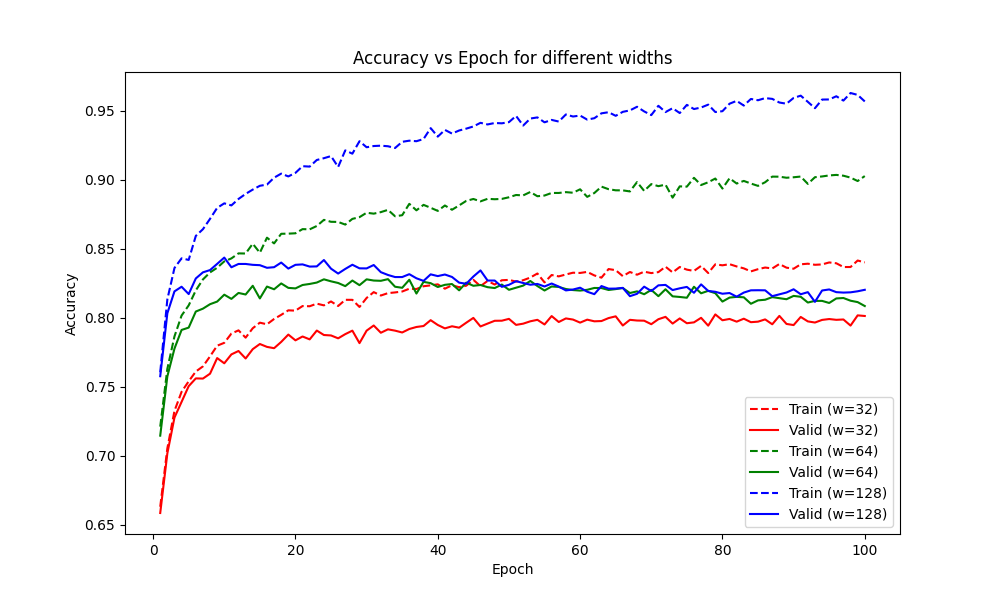
\includegraphics[width=\linewidth]{figures/width_acccurves.png}
        \caption{accuracy by epoch}
        \label{fig:width_acccurves}
    \end{subfigure} 
    \begin{subfigure}{\linewidth}
        \centering
        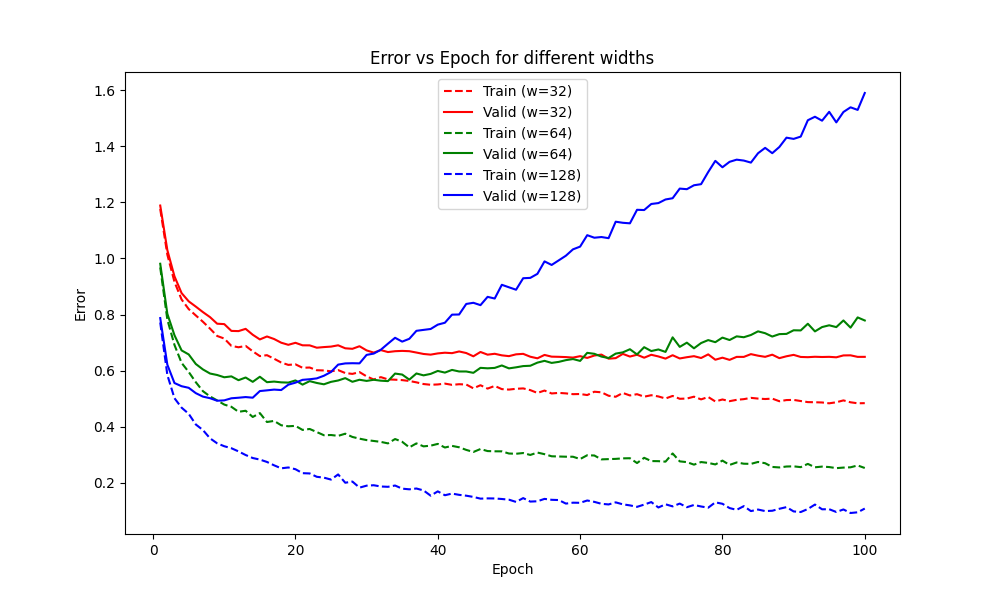
\includegraphics[width=\linewidth]{figures/width_errorcurves.png}
        \caption{error by epoch}
        \label{fig:width_errorcurves}
    \end{subfigure} 
    \caption{Training and validation curves in terms of classification accuracy (a) and cross-entropy error (b) on the EMNIST dataset for different network widths.}
    \label{fig:width}
\end{figure} 
}
}

%% Question Figure 3:
\newcommand{\questionFigureThree} {
\youranswer{Question Figure 3 - Replace these images with figures depicting the accuracy and error, training and validation curves for your experiments varying the number of hidden layers.
%
\begin{figure}[t]
    \centering
    \begin{subfigure}{\linewidth}
        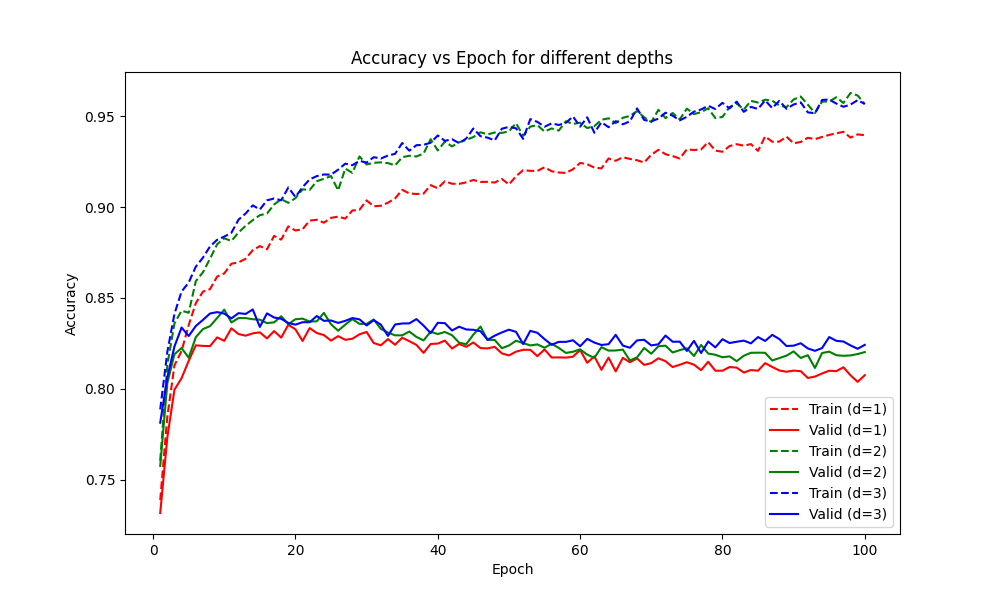
\includegraphics[width=\linewidth]{figures/depth_acccurves.png}
        \caption{accuracy by epoch}
        \label{fig:depth_acccurves}
    \end{subfigure} 
    \begin{subfigure}{\linewidth}
        \centering
        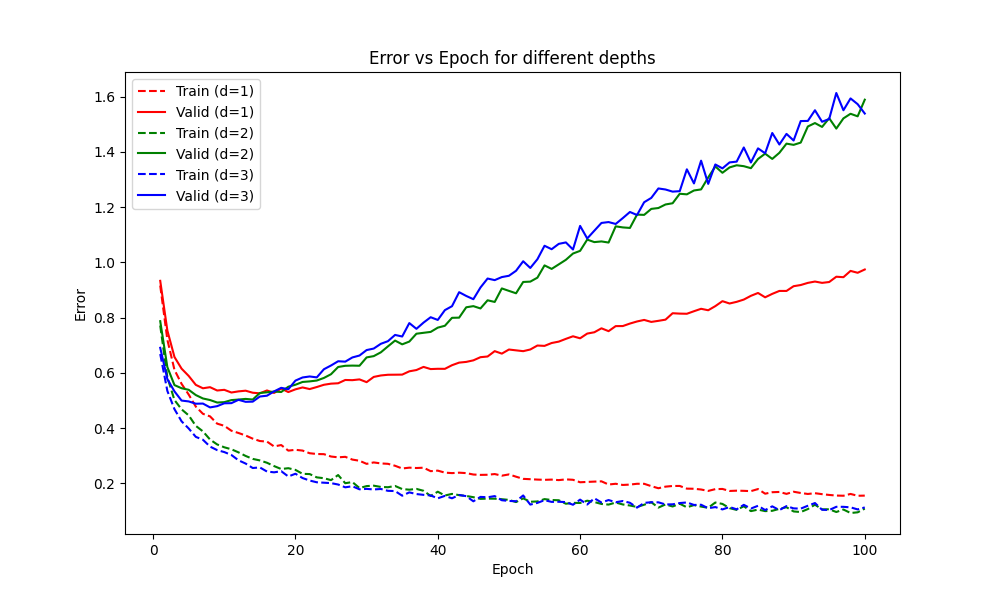
\includegraphics[width=\linewidth]{figures/depth_errorcurves.png}
        \caption{error by epoch}
        \label{fig:depth_errorcurves}
    \end{subfigure} 
    \caption{Training and validation curves in terms of classification accuracy (a) and cross-entropy error (b) on the EMNIST dataset for different network depths.}
    \label{fig:depth}
\end{figure} 
}
}

%% Question Figure 4:
\newcommand{\questionFigureFour} {
\youranswer{Question Figure 4 - Replace these images with figures depicting the Validation Accuracy and Generalisation Gap (difference between validation and training error) for each of the experiment results varying the Dropout inclusion rate, and L1/L2 weight penalty depicted in Table 3 (including any results you have filled in).
%
\begin{figure*}[t]
    \centering
    \begin{subfigure}{.475\linewidth}
        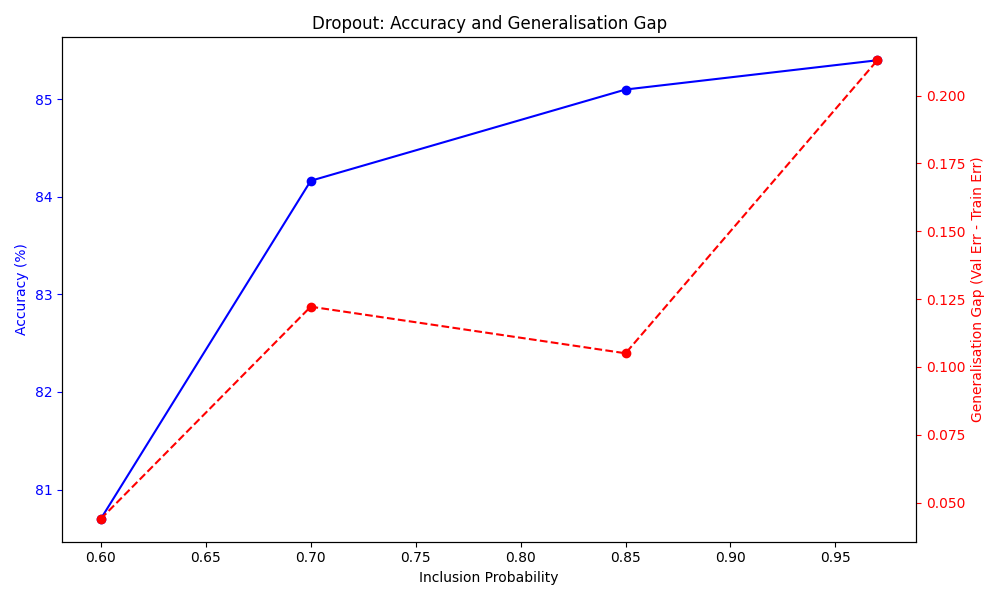
\includegraphics[width=\linewidth]{figures/dropout_plot.png}
        \caption{Accuracy and error by inclusion probability.}
        \label{fig:dropoutrates}
    \end{subfigure} 
    \begin{subfigure}{.475\linewidth}
        \centering
        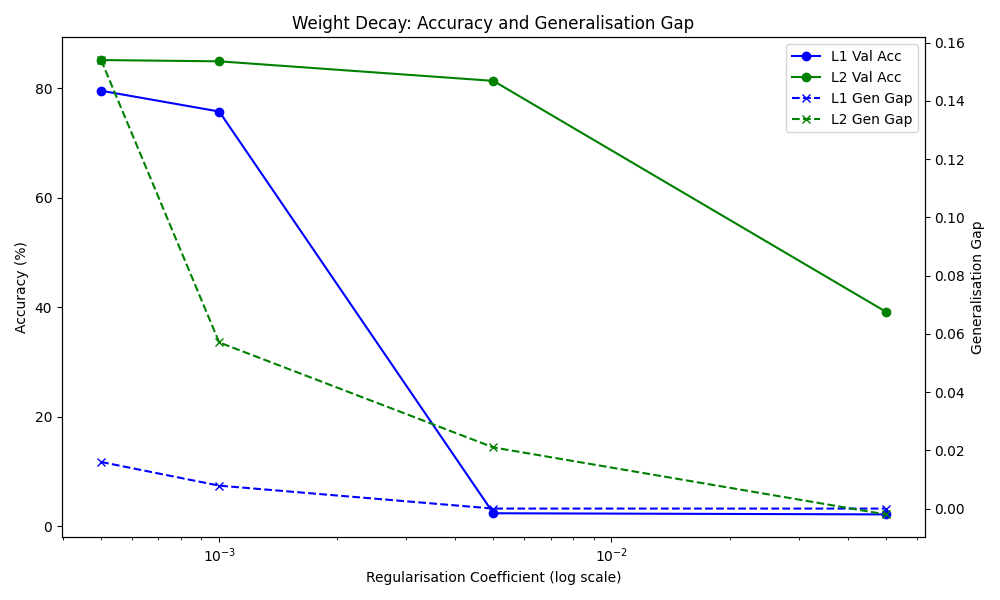
\includegraphics[width=\linewidth]{figures/wd_plot.png}
        \caption{Accuracy and error by weight penalty.}
        \label{fig:weightrates}
    \end{subfigure} 
    \caption{Accuracy and error by regularisation strength of each method (Dropout and L1/L2 Regularisation).}
    \label{fig:hp_search}
\end{figure*}
}
}

%% Question Figure 5:
\newcommand{\questionFigureFive} {
\youranswer{Question Figure 5 - Validation Accuracy and Generalisation Gap for Combined L1/L2 Experiments.
   \begin{figure}[h]
       \centering
       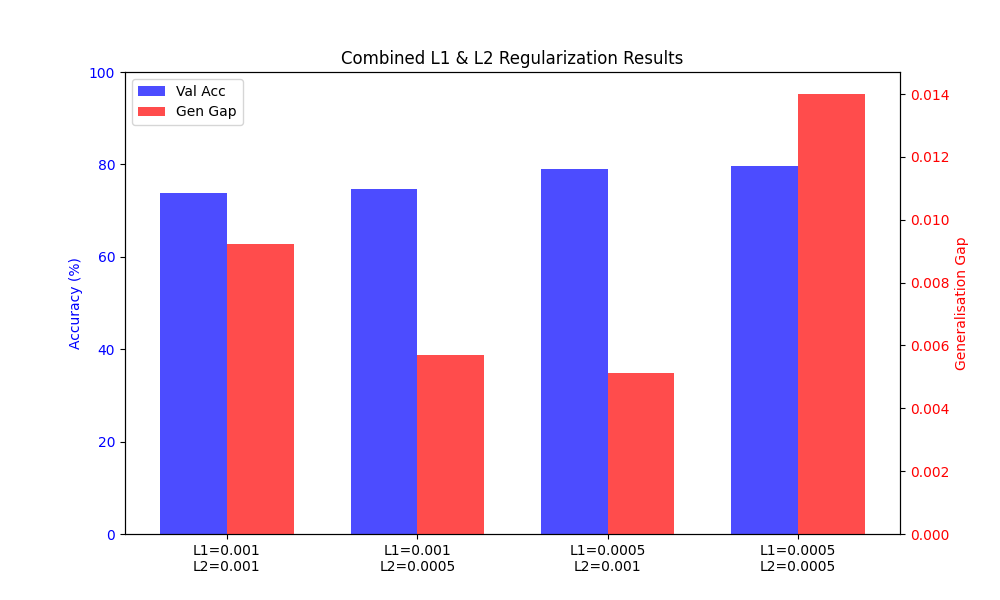
\includegraphics[width=0.8\linewidth]{figures/combined_reg_plot.png}
       \caption{Validation Accuracy and Generalisation Gap for different combinations of L1 and L2 regularization coefficients.}
       \label{fig:l1l2combo}
   \end{figure}
}
}

%% Question Figure 6:
\newcommand{\questionFigureSix} {
\youranswer{Question Figure 6 - Training Accuracy, Error, and Gradient Flow for Custom Activation Function.
   \begin{figure}[h]
       \centering
       \begin{subfigure}{0.32\linewidth}
           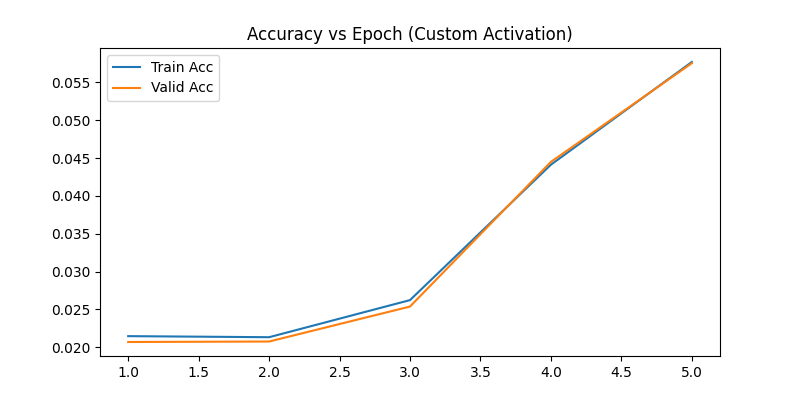
\includegraphics[width=\linewidth]{figures/custom_act_acc.png}
           \caption{Accuracy}
       \end{subfigure}
       \begin{subfigure}{0.32\linewidth}
           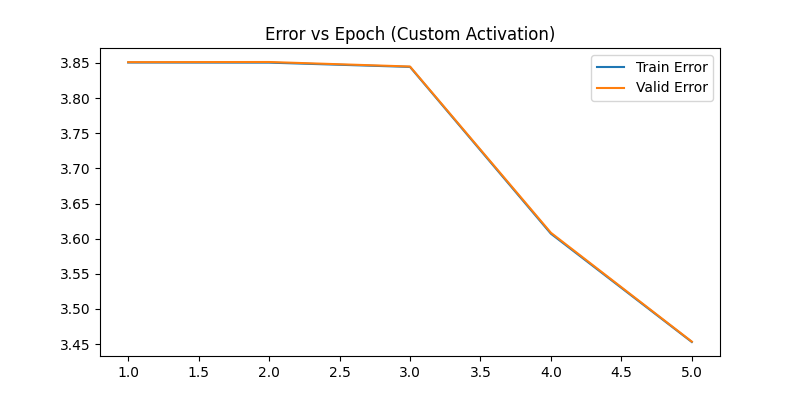
\includegraphics[width=\linewidth]{figures/custom_act_error.png}
           \caption{Error}
       \end{subfigure}
       \begin{subfigure}{0.32\linewidth}
           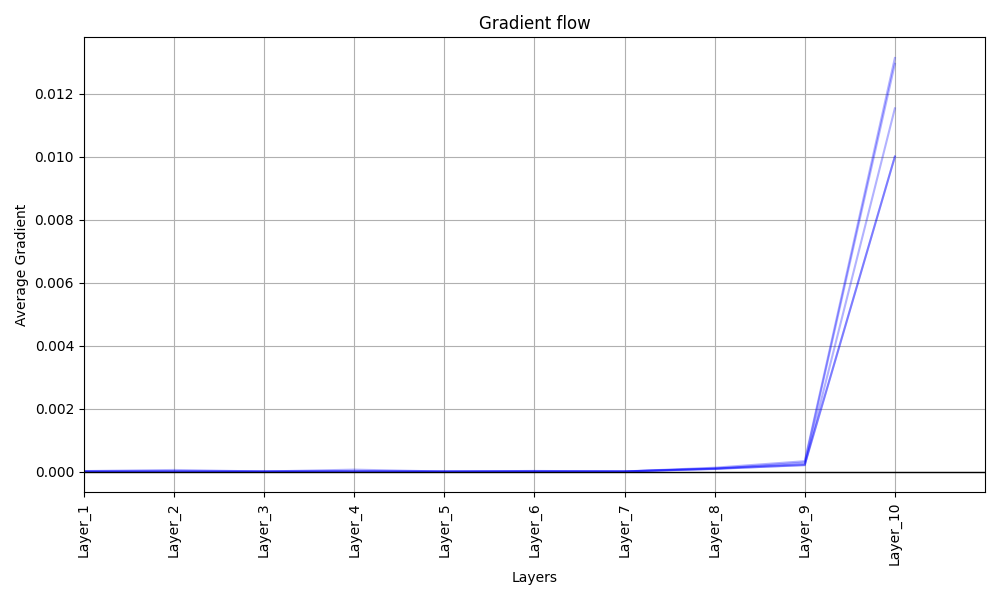
\includegraphics[width=\linewidth]{figures/custom_act_grad_flow.png}
           \caption{Gradient Flow}
       \end{subfigure}
       \caption{Training dynamics for the network with Custom Activation Function.}
       \label{fig:custom_act}
   \end{figure}
}
}

%% - - - - - - - - - - - - TABLES - - - - - - - - - - - - 

%% Question Table 1:
\newcommand{\questionTableOne} {
\youranswer{
Question Table 1 - Fill in Table 1 with the results from your experiments varying the number of hidden units.
%
\begin{table}[t]
    \centering
    \begin{tabular}{c|ccc}
    \toprule
        \# Hidden Units & Val. Acc. & Train Error & Val. Error\\
    \midrule
         32            &    80.12   &  0.484 &   0.649            \\
         64            &    80.84   &  0.253  &   0.779               \\
         128           &    82.02   &  0.109  &   1.589           \\ 
    \bottomrule
    \end{tabular}
    \caption{Validation accuracy (\%) and training/validation error (in terms of cross-entropy error) for varying network widths on the EMNIST dataset.}
    \label{tab:width_exp}
\end{table}
}
}

%% Question Table 2:
\newcommand{\questionTableTwo} {
\youranswer{
Question Table 2 - Fill in Table 2 with the results from your experiments varying the number of hidden layers.
%
\begin{table}[t]
    \centering
    \begin{tabular}{c|ccc}
    \toprule
        \# Hidden Layers & Val. Acc. & Train Error & Val. Error \\
    \midrule
         1               &      80.75      &   0.156 & 0.975                \\
         2               &      82.02      &   0.109 & 1.589                \\
         3               &      82.42      &   0.113 & 1.539                \\ 
    \bottomrule
    \end{tabular}
    \caption{Validation accuracy (\%) and training/validation error (in terms of cross-entropy error) for varying network depths on the EMNIST dataset.}
    \label{tab:depth_exps}
\end{table}
}
}

%% Question Table 3:
\newcommand{\questionTableThree} {
\youranswer{
Question Table 3 - Fill in Table 3 with the results from your experiments for the missing hyperparameter values for each of L1 regularisation, L2 regularisation, Dropout and label smoothing (use the values shown on the table).
%
\begin{table*}[t]
    \centering
    \begin{tabular}{c|c|ccc}
    \toprule
        Model    &  Hyperparameter value(s) & Validation accuracy & Train Error & Validation Error \\
    \midrule
    \midrule
        Baseline &  -                    &               0.837 &       0.241 &  0.533          \\
    \midrule
        \multirow{4}*{Dropout}
                 & 0.6                   &  80.7                &      0.549 & 0.593     \\
                 & 0.7 & 83.0 & 0.450 & 0.515  \\
                 & 0.85 & 85.1 &  0.329 &  0.434 \\
                 & 0.97 & 85.4 &  0.244 & 0.457  \\
    \midrule
        \multirow{4}*{L1 penalty}
                 & 5e-4 & 79.5 & 0.642 & 0.658 \\
                 & 1e-3 & 85.3 & 0.340 & 0.429 \\
                 & 5e-3 & 2.41 & 3.850 & 3.850 \\
                 & 5e-2 & 2.20 & 3.850 & 3.850 \\
    \midrule
        \multirow{4}*{L2 penalty}  
                 & 5e-4 & 85.1 & 0.306 & 0.460 \\
                 & 1e-3 & 85.4 & 0.268 & 0.448 \\
                 & 5e-3 & 81.3 & 0.586 & 0.607 \\
                 & 5e-2 & 39.2 & 2.258 & 2.256  \\
    \midrule
        Label smoothing & 0.1 & 83.9 & 0.911 & 1.207 \\
    \bottomrule
    \end{tabular}
    \caption{Results of all hyperparameter search experiments. \emph{italics} indicate the best results per series (Dropout, L1 Regularisation, L2 Regularisation, Label smoothing) and \textbf{bold} indicates the best overall.}
    \label{tab:hp_search}
\end{table*}
}
}


%% Question Table 4:
\newcommand{\questionTableFour} {
\youranswer{
Question Table 4 - Results for Combined L1 and L2 Regularization.
\begin{table}[h]
    \centering
    \begin{tabular}{cc|ccc}
    \toprule
        L1 Coeff & L2 Coeff & Val. Acc. & Train Error & Val. Error \\
    \midrule
        1e-3 & 1e-3 & \textbf{86.34} & 0.361 & 0.414 \\
        1e-3 & 5e-4 & 85.34 & 0.358 & 0.441 \\
        5e-4 & 1e-3 & 81.40 & 0.585 & 0.607 \\
        5e-4 & 5e-4 & 79.55 & 0.642 & 0.656 \\
    \bottomrule
    \end{tabular}
    \caption{Validation accuracy (\%) and training/validation error for combined L1 and L2 regularization.}
    \label{tab:l1l2_exp}
\end{table}
}
}

%% END of YOUR ANSWERS